\chapter{Real-Time Implementation}
JUCE
Give overall structure of code


Implementation of the physical models
using FDTD methods

As mentioned in Chapter \ref{ch:physMod}, FDTD methods are used for high-quality and accurate simulations, rather than for real-time applications. This is due to their lack of simplifications.

Usually, \texttt{MATLAB} is used for simulating 

Here, an interactive application is considered real-time when
\begin{center}\it
    Control of the application generates or manipulates audio with no noticeable latency.
\end{center}

Also the application needs to be controlled continuously

Helps to (informally) evaluate the models by interacting with it in a natural way (rather than static parameters)

\section{MATLAB vs. C++}
It is usually a good idea to prototype a physical modelling application in MATLAB for several reasons:
\begin{itemize}
    \item Easier to debug
    \begin{itemize}
        \item Plotting functionality
        \item No need for memory handling
    \end{itemize}
    \item Instability due to programming errors 
\end{itemize}

\subsection{Speed}
Here is where the power of C++ 



\subsection{Syntax}
Indexing in
Matlab is 1-based, meaning that the index of a vector starts at 1. If \texttt{u} is a vector with 10 elements, the first element is retrieved as \texttt{u(1)} and the last as \texttt{u(10)}. C++, on the other hand, is 0-based and retrieving the first and last element of a size-10 vector happens through \texttt{u[0]} and \texttt{u[9]}respectively. 

\section{Do's and don'ts in Real-Time FD schemes}
Some of the things I learned (the hard way)...
\begin{itemize}
    \item Create a limiter
    \item Structure your application into classes 
    \item Use pointer switches
    \item Comment your code (hehe)
\end{itemize}

\subsubsection{Create a limiter}
Programming errors happen. To save your speakers, headphones or -- most importantly -- your ears, create a limiter. 

\setlstCpp
\begin{lstlisting}
double limit (double val)
{
    if (val < -1)
    {
        val = -1;
        return val;
    }
    else if (val > 1)
    {
        val = 1;
        return val;
    }
    return val;
}
\end{lstlisting}

\setlstMAT
\begin{lstlisting}
for  i = 0:lengthSound
    uNext = ...
end
\end{lstlisting}

\subsubsection{Use pointer switches}
One of the most important things in working with FD schemes for real-time audio applications is to 

The maximum number of copy-operations this takes is $2(N+1)$ if the boundaries also need updated in the case of free or Neumann boundary conditions. For a string with simply supported or clamped boundary conditions this can be reduced to $2N$ or $2(N-1)$ respectively, but does not maka big difference in computational time. 

A pointer switch, however, only needs 4 copy-operations per iteration as shown in Algorithm \ref{lst:cppPointer} 

\begin{figure}[h]
    \subfloat[Copying values: $2(N+1)$ operations per iteration. \label{fig:vectorCopy}]{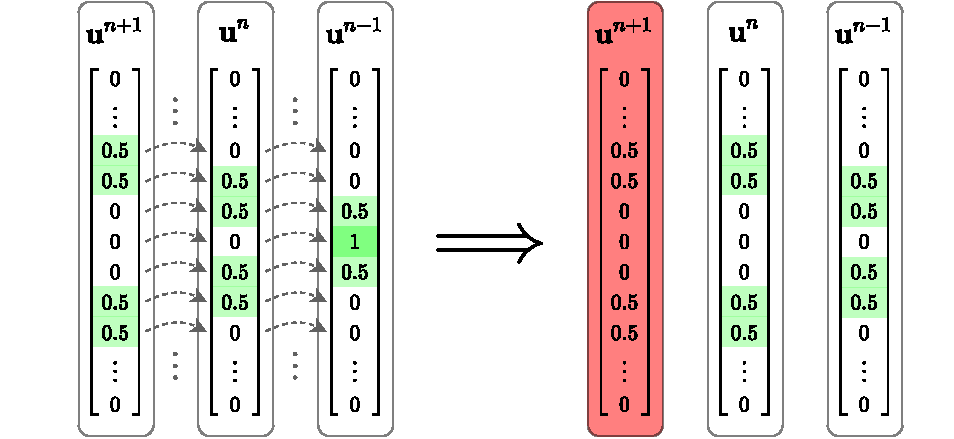
\includegraphics[width=\textwidth]{figures/realtime/vectorCopy.pdf}}\\
    \subfloat[Pointer switch: 4 operations per iteration. \label{fig:pointerSwitch}]{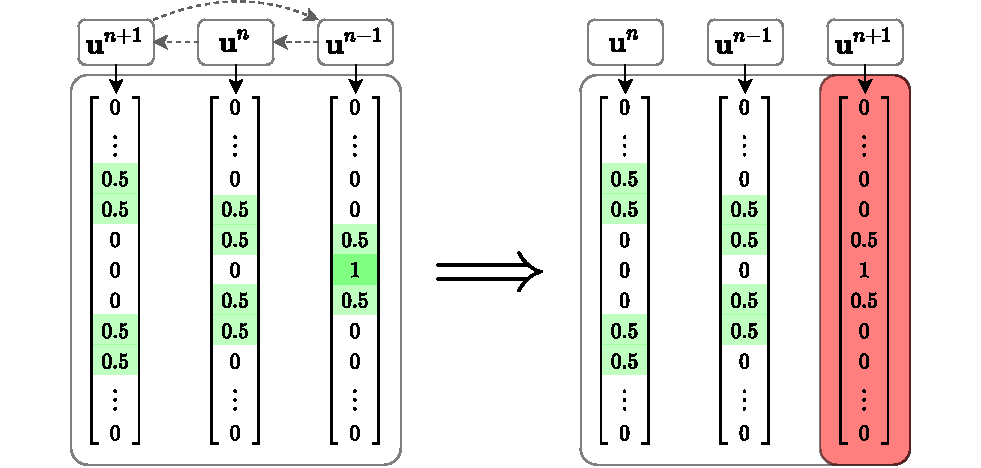
\includegraphics[width=\textwidth]{figures/realtime/pointerSwitch.pdf}}
    \caption{Updating the state vectors by (a) copying all values individually, or (b) performing a pointer switch. Non-zero values are highlighted in green for clarity. The values of the red vector will be overwritten by the update of the scheme in the next iteration so these values will no longer be used.}
\end{figure}


\setlstMAT
\begin{lstlisting}
for n = 1:lengthSound
    ...
    uPrev = u;
    u = uNext;
end
\end{lstlisting}



In C++ this is done using
\setlstCpp
\begin{lstlisting}[caption=Implementation of a pointer switch also shown in Figure \ref{fig:pointerSwitch}. A temporary pointer is assigned to where the $\u^{n-1}$ pointer is currently pointing at to be able to assign that location in memory to the $\u^{n+1}$ pointer in the end., label=lst:cppPointer]
double updateStates()
{
    double* uTmp = u[2];
    u[2] = u[1];
    u[1] = u[0];
    u[0] = uTmp;
}
\end{lstlisting}

\pagebreak
\subsubsection{Grouping terms and Precalculating coefficients}
Generally in implementations of FD schemes the most computationally expensive part of the algorithm is the calculation of the scheme itself. This is due to the rate at which it needs to be updated which usually is 44100 Hz. Graphics can be updated at rates orders of magnitude lower than the audio (say 10-20 Hz) and still be considered smooth enough.

A more compact way to write the 1D wave update equation in Eq. \eqref{eq:1DwaveUpdate} is 
\begin{equation}\label{eq:1DwaveUpdateCompact}
    u_l^{n+1} = (2 - 2 \lambda^2) \uln - u_l^{n-1} + \lambda^2\left(u_{l+1}^n + u_{l-1}^n\right).
\end{equation}
Grouping the terms like this allows for the coefficients multiplied onto the grid function at different temporal and spatial indices to be precomputed. This can significantly decrease the amount of operations per sample.

The undamped stiff string FD scheme%in \eqref{eq:stiffStringFDS}
\begin{equation}
    \dtt \uln = c^2 \dxx \uln - \kappa^2 \dxxxx \uln,
\end{equation}
can be expanded to an update equation as
\begin{equation}
    \begin{aligned}
        u_l^{n+1} = &\ 2\uln - u_l^{n-1} + \lambda^2 \left(u_{l+1}^n - 2\uln + u_{l-1}^n\right)\\
        & - \mu^2 \left(u_{l+2}^n - 4u_{l+1}^n + 6\uln + -4u_{l-1}^n + u_{l-2}^n\right)
    \end{aligned}
\end{equation}
where $\lambda = ck/h$ and $\mu = \kappa k / h^2$.

For implementation purposes there is a better way to write this scheme that reduces the amount of computations. This is done by collecting the terms based on the grid function and pre-calculating the coefficients multiplied onto these. As the schemes are spatially symmetric, ``neighbouring points'' relative to $\uln$ can also be grouped to get
\def\semilarge{\fontsize{11}{11.6}\selectfont}
\begin{equation}
    u_l^{n+1} = \underbrace{(2 - 2\lambda^2 - 6\mu^2)}_{\texttt{\semilarge B1}}\uln  + \underbrace{\left(\lambda^2 + 4\mu^2\right)}_{\texttt{\semilarge B2}}\left(u_{l+1}^n+u_{l-1}^n\right)\underbrace{-\mu^2}_{\texttt{\semilarge B3}} \left(u_{l+2}^n+u_{l-2}^n\right) \underbrace{-}_{\texttt{\semilarge C1}} u_l^{n-1}.
\end{equation}
These coefficients can then be pre-calculated and do not have to be 

\begin{lstlisting}[caption=Precalculation]
//// Constructor ////
B1 = 2.0 - 2.0 * lambdaSq - 6.0 * muSq; // u_l^n
B2 = lambdaSq + 4.0 * muSq;             // u_{l+-1}^n
B3 = -muSq;                             // u_{l+-2}^n
C1 = -1.0;                              // u_l^{n-1}

//// Function where scheme is calculated ////
for (int l = 2; l < N-1; ++l) // clamped boundaries
{
    u[0][l] = B1 * u[1][l]
            + B2 * (u[1][l+1] + u[1][l-1]) 
            + B3 * (u[1][l+2] + u[1][l-2])
            + C1 * u[2][l];
}
\end{lstlisting}

\section{Graphics}
\setlstCpp
\begin{lstlisting}
void Simple1DWave::paint (juce::Graphics& g)
{
    // clear the background
    g.fillAll (getLookAndFeel().findColour (juce::ResizableWindow::backgroundColourId));
    
    Path stringState = visualiseState (g, 100);
    
    // choose your favourite colour
    g.setColour (Colours::cyan);
    
    // visualScaling depends on your excitation
    g.strokePath (visualiseState (g, 100), PathStrokeType(2.0f));
    
}

Path Simple1DWave::visualiseState (Graphics& g, double visualScaling)
{
    // String-boundaries are in the vertical middle of the component
    double stringBoundaries = getHeight() / 2.0;
    
    // initialise path
    Path stringPath;
    
    // start path
    stringPath.startNewSubPath (0, -u[1][0] * visualScaling + stringBoundaries);
    
    double spacing = getWidth() / static_cast<double>(N);
    double x = spacing;
    
    for (int l = 1; l <= N; l++)
    {
        // Needs to be -u, because a positive u would visually go down
        float newY = -u[1][l] * visualScaling + stringBoundaries;
        if (isnan(x) || isinf(abs(x)) || isnan(u[1][l]) || isinf(abs(u[1][l])))
            std::cout << "Wait" << std::endl;
        
        // if we get NAN values, make sure that we don't get an 
        // exception
        if (isnan(newY))
            newY = 0;
        
        stringPath.lineTo (x, newY);
        x += spacing;
    }
    
    return stringPath;
}
\end{lstlisting}
\pagebreak
\begin{lstlisting}
void Simple1DWave::excite()
{
    //// Raised cosine excitation ////
    
    // width (in grid points) of the excitation
    double width = 10;
    double excitationLoc = 0.2;
    // make sure we're not going out of bounds at the left boundary
    int start = std::max (floor((N+1) * excitationLoc) - floor(width * 0.5), 1.0);
    
    for (int l = 0; l < width; ++l)
    {
        // make sure we're not going out of bounds
        // at the right boundary (this does 'cut off'
        // the raised cosine)
        
        if (l+start > N - 1)
            break;
        
        u[1][l+start] += 0.5 * (1 - cos(2.0 * double_Pi * l / (width-1.0)));
        u[2][l+start] += 0.5 * (1 - cos(2.0 * double_Pi * l / (width-1.0)));
    }
}
    
\end{lstlisting}